\chapterauthor{thomas mcandrew}{Lehigh University}
%\chapterauthor{Second Author}{Second Author Affiliation}
\chapter{Sets, the sample space, and probability}
\hspace{1mm}

\section{Introduction}\label{intro}

When we decide to study a topic, we often have in mind a \text{population}, a protocol to observe members of our population, a hypothesis that posits some aspects of our observed members.
We collect data, we compile results.
At the close of our study we want to know how the results ("what happened") contribute to our hypotheses ("what we thought may happen") and, importantly, the chances that if we reproduced the same study that the results would lead us towards the same conclusions.  

For example, suppose we decide to study the impact of percutaneous intervention (PCI) versus optimal medical therapy (OMT) to treat patients how have had a myocardial infarction, often called a "heart attack".
Patients are enrolled in a study and randomly assigned PCI or OMT.
We hypothesize that PCI will result in a prolonged life from when the intervention took place onward.
After our study we find patients who underwent PCI live on average 100 days longer than those who underwent OMT. 
However, it feels unsatisfactory to have a single number describing how effective PCI was at prolong life. 
We may want to know the chances PCI prolongs life 80 days, 30 days, or maybe zero days, compared to OMT. 

We want to understand how likely we are to see specific events.
The formal method of assigning chances to a set of events is called probability theory.

\section{Probability lingo}
\hspace{1mm}
%Sets, Outcomes, Events, and the Sample space
\subsection{Sets}

We define a \textbf{set} as a collection of items, sometimes called elements. 
A set is typically given a capital letter (for example $A$) and the elements are included inside curly braces. 

Here, we define three sets
\begin{align}
    A &= \{ a,b,c\}\\
    C &= \{ -1,1,3.14\}\\
    Z &= \{ \text{orange},1,\text{puppy dog}\}
\end{align}
The elements inside a set are unordered and do not necessarily need to be numbers. A set can contain any object.
The set $A$ could have been defined as $\{a,b,c\}$ or $\{c,b,a\}$.
We use the symbol $\in$ to express that an element "is a member of" a set.
For example, $a \in A$ can be read "the element a is a member of the set A" or "the element a is in the set A". 
We can also communicate when an element is not a member of a set with the symbol $\notin$.
For example, $c \notin C$ is read "the element c is not a member of (not in) the set C".

\textbf{Generating sets:} We can define a set by enclosing in brackets each individual element. $S = \{a,b,c,10\}$.
However, some sets may be easier to build with properties.
A property is a function from elements to either true or false. 
For example we could define the property $P(x) = 1 \text{ when } x \text{ is even and } 0 \text{ when } x \text{ is odd}$. 
To build a set that contains elements with a specific property, we write
$S = \{x | P(x)\}$ or $S = \{x | x \text{ is an even integer} \}$. 
This is read "the elements $x$ such that $x$ is an even integer".
The vertical bar replaces the words "such that".

Two sets are \textbf{equal} is they contain the same elements.
In other words, if for an element $x$, $x \in A$ implies that $x \in B$ \textbf{and} if for an element $y$, $y \in B$ implies that $y \in A$ then the set $A$ and set $B$ are equal.
If a set $A$ and set $B$ are equal we write $A=B$. 
If two sets do not contain the same elements then they are \textbf{unequal} and we write $A \neq B$.

Lets look at an example.
\begin{align}
    A &= \{ a,b,c\}\\
    B &= \{ b,a,c\}\\
    C &= \{ b,c\}
\end{align}
Above, $A=B$ but $A \neq C$ and $B \neq C$.

A set $A$ is a \textbf{subset} of a second set $B$ if all of the elements in $A$ are also elements in $B$.
We can say that $A$ is a subset of $B$ if every element in $x$ implies that element is in $B$, or $x \in A$ implies $x \in B$.
We write $A \subset B$ to denote that $A$ is a subset of $B$. 
To denote that a set $A$ is \textbf{not a subset} of $B$, we write $A \not\subset B$. 
In the example above, the $C$ is a subset of $A$ $C \subset A$, but $A$ is not a subset of $C$, or $A \not\subset C$.

We can build new sets by operating on two or more existing sets.

Set \textbf{intersection} takes as input two or more sets, $A$,$B$, and returns a set that contains all the elements that are in both $A$ \underline{and} $B$.
We use the symbol "cap" to denote set intersection $A \cap B$ and often say "A intersect B". 

For the above sets $A$ and $C$, their intersection is 
\begin{align}
    A \cap C = \{c,b\}
\end{align}
because the element $c$ belongs to both set $A$ and set $C$ and because the element $b$ belongs to $A$ and $C$.

We can intersect more than two sets. 

Let $A =\{ a,b,10,12 \}$, $Z =\{ b,10,-1 \}$, $U =\{ a,b,c,d,10 \}$.
Then
\begin{equation}
    A \cap Z = \{ b,10 \}    
\end{equation}
and 
\begin{equation}
 A \cap Z \cap U = \{ b,10\}.
\end{equation}

If $A$ is a subset of $B$, $A \subset B$, then the only elements both sets have in common are those in $A$. 
The intersection of $A$ and $B$ is then
\begin{align}
    \begin{aligned}
      \text{If } A \subset B \text{ then}\\
       A \cap B = A.
    \end{aligned} \label{subsetInter}
\end{align}

Set \textbf{union} takes as input two or more sets and output a set that contains all the elements that belong to first set \underline{or} the second set \underline{or} the third set, and so on.
We use the "cup" symbol to denote set union. 
As an example, consider the sets $A$, $Z$, and $U$ to be the same as they are above. 
Then $A$ \textbf{union} $Z$ is 
\begin{equation}
    A \cup Z = \{a,b,10,12,-1\}
\end{equation}
This is because each of the above elements belongs to at least one of the sets $A$ and $Z$. As another example, 
\begin{equation}
    A \cup Z \cup U = \{a,b,c,10,12,-1\}
\end{equation}

Intersection and union are the most common set operations. 
Before we define the set operation \textbf{complement}, we need to discuss two special sets. 

The \textbf{universal set} is the set of all elements. 
We denote the universal set with a $\mathcal{G}$.
The set which contains no elements is called the \textbf{empty set}, and we denote the empty set as $\emptyset$.

If a set $A$ and set $B$ have no elements in common, then $A \cap B = \emptyset$.
We often say that the set $A$ and $B$ are \textbf{disjoint}.
For example, 
\begin{align}
    \begin{aligned}
       A = \{ 1,3,5 \} \\
       Q = \{ 2,4,6 \} \\
       A \cap Q = \emptyset
    \end{aligned}
\end{align}
Because the intersection between $A$ and $Q$ is empty, these sets are disjoint.

Now for our final set operation---complement.
The set complement takes as input a single set, $A$, and outputs a set with elements that are members of $\mathcal{G}$ but are not members of $A$.
We denote set complement in one of two ways: $A^{c}$ or $A'$.

\begin{VT1}

\VH{Set operations example}
Let's look at an example of how these sets and set operations work. 
Define the universal set, $\mathcal{G}$, to be the set of all positive integers (i.e. $1,2,3,4,\cdots$). Lets define the sets $A_{1}=\{1\},A_{2}=\{1,2\},A_{3}=\{1,2,3\}, \cdots, A_{n}=\{1,2,3,4\cdots,n\} $. We use a subscript and a number to "index" our sets. 
An index is an easy way to keep track of sets (and many mathematical objects).
\begin{align}
    \begin{aligned}
        A_{1} \cap A_{2} &= \{ 1 \}\\
        A_{1} \cap A_{5} &= \{ 1 \}\\
        A_{3} \cap A_{8} &= \{ 3 \}\\
    \end{aligned}
\end{align}
Note that $A_{3} \cap A_{8}$ is not the value $3$, but the set \{3\}.
The examples above suggest a pattern for any set $A_{i}$ and $A_{j}$ where $i \leq j$:
\begin{align}
    A_{i} \cap A_{j} = \{ i \}
\end{align}

Lets look at set union in this example
\begin{align}
    \begin{aligned}
        A_{1} \cup A_{2} &= \{ 1,2 \}\\
        A_{1} \cup A_{5} &= \{ 1,2,3,4,5 \}\\
        A_{3} \cup A_{8} &= \{ 1,2,3,4,5,6,7,8 \}\\
    \end{aligned}
\end{align}
and we see the following pattern for $i \leq j$
\begin{align}
    A_{i} \cup A_{j} = \{1,2,3,4\cdots,j \} = A_{j}
\end{align}

Because we defined a universal set, we can look at set complement
\begin{align}
    \begin{aligned}
        A_{1}^{c} &= \{2,3,4,5,\cdots \}\\
        A_{5}^{c} &= \{6,7,8,9\cdots \}\\
        A_{8}^{c} &= \{9,10,11,12,\cdots \}\\
    \end{aligned}
\end{align}
\end{VT1}

\section{Applying set theory to probability}
\vspace{-0.75cm} \hspace{1mm}  
\subsection{Foundation}
The ideas about sets and set operations are the foundations for how we think about probability, about experiments, and hypotheses. 
We only need to recast the above set ideas to results from an experiment. 

We use $\mathcal{G}$ to define the set of all possible outcomes from an experiment and call this set the \textbf{sample space}. 
The term "experiment" has a broad meaning. 
An experiment can mean everything from a randomized controlled trial to an observational study.
Here an \textbf{experiment} is the process that generates outcomes.

An \textbf{outcome} is defined as an element of the sample space. 
An outcome is a single observation from an experiment, and we define an \textbf{event} as a set of outcomes. 
Most often we use $o_{i}$ to denote an outcome and $E_{i}$ to denote an event.

The \textbf{probability} of an event $E$ is a mapping from the set $E$ to a number between, or equal to, the values 0 and 1. We use $P(E)$ to denote the probability of event $E$.
We require that the probabilities assigned to individual sets consisting of a single element in $E$ add up to the probability of $E$. 
Lets suppose there are $n$ outcomes in the event $E$.
Then
\begin{align}
    \begin{aligned}
       E &= \{ o_{1}, o_{2}, o_{3}, \cdots, o_{n}\} \\ 
       P(E) &= P(\{o_{1}\}) + P(\{o_{2}\}) \cdots P(\{o_{n}\})
    \end{aligned}
\end{align}

We further require $P(\mathcal{G}) = 1$.
In other words, the probability that something happens is certain.
Note that we do not need to describe how we assign probabilities to events, we only describe what values we expect those numbers to be.

Lets further detail relationships between probabilities of sets that we would expect. 
\begin{enumerate}
    \item If $A \subset B$ then $P(A) \leq P(B)$ \label{subsetrule}. 
    \item $P(A \cup B) \leq P(A) + P(B)$ (why?)
    \item $P(A \cup B) = P(A) + P(B) - P(A \cap B)$
    \item If $A$ and $B$ are disjoint then $P(A \cup B) = P(A) + P(B) $
\end{enumerate}

The following three axioms (knowledge we assume true without proof) are called \textbf{Kolmorogov's axioms} ($\label{KA}$)
\begin{enumerate}
    \item For any event $E$, $P(E) \geq 0$
    \item $P(\mathcal{G}) = 1$
    \item If $E_{1}$ and $E_{2}$ are disjoint then $P(E_{1} \cup E_{2}) = P(E_{1}) + P(E_{2})$
\end{enumerate}

\textbf{Example:} When we want to compute the probability that an outcome fall in any one of the events, say $E_{1}, E_{2},E_{3}$, knowing that these events have no outcomes in common, that they are disjoint, makes the computation easy. An intuitive way to think about events that are disjoint is if they cannot all occur at the same time.
Suppose we wish to study the prevalence of stroke among patients who are older than sixety-five.
Strokes can be categorized into transient ischemia attacks (TIA), ischemic stroke (IS), and hemorrhagic stroke (HS).
Further lets assume the following probabilities for each event: $P(\{\text{TIA}\}) = 0.15$, $P(\{\text{IS}\}) = 0.75$, $P(\{\text{HS}\}) = 0.10$, and that these events cannot occur simultaneously. Then the probability of the event $E=\{TIA,HS\}$ can be broken into the union of two disjoint events $E = \{TIA\} \cup \{HS\}$ and we can use what we know about these disjoint events to compute the probability of $E$
\begin{align}
    P(E) &= P(\{\text{TIA},\text{HS}\} ) \\ 
         &=P(\{\text{TIA}\} \cup \{\text{HS}\} ) \\
         &=P(\{\text{TIA}\}) + P(\{\text{HS}\} ) \;\;\;\text{disjoint} \\
         &= 0.15 + 0.75 = 0.90
\end{align}

\subsection{The principle of equally likely outcomes---one way to assign probabilities}

There are many different ways to assign probabilities to events. 
In this text, we will only consider using the principle of equally likely outcomes to assign probabilities. 
The \textbf{principle of equally likely outcomes} (PELO) states that the probability we assign to every event which contains a single outcome, $E_{i} = \{o_{i}\}$, in a sample space $\mathcal{G}$ is equal.

We can use this principle to assign probabilities first to every individual outcome and then to arbitrary events. Assume the PELO is true, then 
\begin{align}
    o_{1},o_{1},o_{1}, \cdots,o_{n} \in \mathcal{G}\\
    E_{i} = \{o_{i}\}\\
    E_{1} \cup E_{2} \cup E_{3} \cup \cdots \cup E_{n} = \mathcal{G} \;\; \text{(why?)}\\ 
    P(E_{1} \cup E_{2} \cup \cdots \cup E_{n}) = P(\mathcal{G}) = 1 \\ 
    P(E_{1} \cup E_{2} \cup \cdots \cup E_{n}) = P(E_{1}) + P(E_{2} \cup \cdots \cup E_{n}) \;\; (\text{disjoint})\\
    P(E_{1}) + P(E_{2}) + \cdots P(E_{n}) = 1\\
    n \cdot p = 1 \;\; (p \text{ is the constant prob. we are after})\\
    p = 1/n
\end{align}
The PELO tells us that the probability of an event with a single outcome is equal to one divided by the total number of outcomes in the sample space.
The PELO also tells us that for a sample space with $n$ elements the probability of an event $E = \{o_{1},o_{20},o_{4}\}$ that contains three outcomes is $P(E) = \frac{3}{20}$.


\begin{VT1}

\VH{An example when, and when not, the PELO applies.}

PELO only works when we expect each outcome in our sample space to be equally likely.\\ 

\textbf{Example 1} Suppose our experiment is a coin toss and we will observe whether or not the coin lands heads up (H) or tails up (T). If we assume the coin has not been altered in any way, then PELO applies.
Our sample space is $\mathcal{G} = {H,T}$. 
Because there are two outcomes in our sample space, $P(\{H\}) = 1/2$ and $P(\{T\}) = 1/2$.

\textbf{Example 2} Suppose for our experiment we observe for one year a single patient who was admitted to the hospital because of an influenza infection and we plan to observe if that patient returns to the hospital because of a second infection. Our sample space contains one outcome $R$ if the patient is re-admitted to the hospital within one year and a second outcome if they are no re-admitted ($N$).
Our sample space is $\mathcal{G} = {R,N}$. 
If we applied the PELO to this problem we would have to assume the probability this patient returns, or does not return, are equal. Intuitively,it feels unreasonable to assume these two events have equal probabilities.

We need an additional way to assign probabilities.
\end{VT1}

\subsection{A frequentist approach to assigning probabilities}

An empirical approach to assign probabilities to an event $A$ with sample space $\mathcal{G}$ is to do the following:
\begin{enumerate}
    \item Generate $1, 2, 3, 4, \cdots, N$ outcomes from $\mathcal{G}$
    \item Define a variable $N(A)$ and set that variable to zero.
    \item If the 1st outcome is a member of $A$ than add one $N(A)$, otherwise move on
    \item If the 2nd outcome is a member of $A$ than add one to $N(A)$\\
    \vdots
    \item If the Nth outcome is a member of $A$ than add one to $N(A)$
\end{enumerate}
The above algorithm defined a variable $N(A)$ that counts the number of outcomes that belong to $A$ out of the $N$ generated outcomes.
We can assign to $A$ the probability 
\begin{equation}
    P(A) = \frac{N(A)}{N}
\end{equation}
that is, the number of times we observed an outcome that belonged to A divided by the number of outcomes we observed.

As an example, suppose we want to understand the probability that patients with non-medically treated type II diabetes transition to needing treatment within one year of their diagnosis.
Our outcomes are $\mathcal{G}$ = \{"need treatment" and "no treatment"\}. 
To assign a probability to the event $E = \{\text{need treatment}\}$ using the frequentist approach we decide to request anonymized patient records from a set of hospitals, asking that each hospital only send those patients who had an original diagnosis of type II diabetes without medication and who have had a physician visit one year more later.
After our data request, we received 5,000 patient records and find that 1,585 of these patients were asked to start medication for their type II diabetes within one year.
A frequentist approach would assign
\begin{equation}
    P(E) = 1,585/5,000 = 0.317
\end{equation}
and also assign to the event $F=\{\text{no treament}\}$
\begin{equation}
    P(F) = 0.683 \; \; \text{(why?)}
\end{equation}.

\subsection{Products, Conditionals, Baye's Theorem, and Repeated Experiments }
\hspace{1mm}

\subsubsection{Product Sets}

Suppose a novel vaccine was developed and we are asked to compare two probabilities: the probability a vaccinated patient is infected before 30 days after they receive their vaccine and the probability a patient who has not received a vaccine is infected before 30 days since they have enrolled in the experiment. 
To estimate these probabilities, we enroll 200 volunteer patients. We will assign 100 patients to be given the treatment and the remaining 100 patients will be observed without treatment.

Because of our experimental design, $P(\{\text{vaccinated}\})=1/2$ and $P(\{\text{not vaccinated}\}) = 1/2$ with a sample space $\mathcal{G_{\text{assignment}}}$, containing two outcomes $\{\text{vaccinated},\text{not vaccinated}\}$.
But our main interest is in the probability of infection within 30 days of enrolling in the study, and so our main interest is in the a related sample space $\mathcal{G}_{\text{infection}} = \{\text{infection}, \text{no infection}\}$.
We need a way to combine these sample spaces together so that we can estimate the probability of a patient that is vaccinated \underline{and} that is infected. 

Up until this point we have learned how to assign probabilities to events in one sample space. 
Lets look at how we may assign events to a combination of, and later a sequence of, sample space\textbf{s}.

\textbf{Products of sets:}   
First, we'll need to talk about the product of two sets. 
Let $A = \{a,b,c\}$ and $B = \{1,2,3\}$. 
Then the Cartesian product $C = A \times B$ is a set where each element in $A$ is paired with each element in $B$. 
\begin{equation}
    C = \{(a,1),(a,2),(a,3),(b,1),(b,2),(b,3),(c,1)(c,2)(c,3)  \}
\end{equation}
We use the notation $(,)$, called a "tuple", to denote pairs.
A \textbf{tuple} is an outcome belonging to a sample space built from the Cartesian product of many individual sample spaces. 
Tuples are ordered. The tuple $(a,1) \neq (1,a)$.
The above is called a Cartesian product because you could imagine creating a grid where the horizontal axis has gridlines at "a", "b", "c" and the vertical axis has grid lines at "1", "2", and "3". Where the gridlines intersect are the tuples that belong to $C$.

We can apply the Cartesian product to combine samples spaces.
Define $\mathcal{G}_{\text{experiment}}$ as the Cartesian product between $\mathcal{G}_{\text{assignment}}$ and $\mathcal{G}_{\text{infection}}$, or 
\begin{equation}
    \mathcal{G}_{\text{experiment}} = \mathcal{G}_{\text{assignment}} \times \mathcal{G}_{\text{infection}}
\end{equation}
This new sample space has the following outcomes:
\begin{align}
   \begin{aligned}
   \mathcal{G}_{\text{experiment}} = \{(\text{vaccinated},\text{infection}),(\text{vaccinated},\text{not infected}) \\
   ,(\text{not vaccinated},\text{infection}),(\text{not vaccinated},\text{not infected})\}
   \end{aligned}
\end{align}
Our new sample space has $4$ outcomes, two outcomes from the assignment sample space are paired with two outcomes from the infection sample space ($2$ outcomes $\times$ $2$ outcomes equals $4$ outcomes in the new space).

With this new space in hand, we can assign probabilities to the outcomes "vaccinated \underline{and} infected" and the outcome "not vaccinated \underline{and} infected".
You may hear events like the above called \textbf{compound events}, or \textbf{joint events}.

Let's use the frequentist approach to estimate the probabilities of these four events.
We enroll all 200 patients over a 6 months period and then follow each patient for 30 days. 
At 7 days, 14 days, 21 days, and at the end of there 30 day period they meet with a physician to relay information about how they feel that could indicate they had an infection.
We collect the following data:

\begin{table}[ht!]
    \centering
    \begin{tabular}{cccc}
        \hline
        Vaccinated & Infected & Frequency & Estimated Prob.\\
        \hline
         Yes & Yes &  20 & 20/200 = 0.1 \\
         Yes & No  &  80 & 80/200 = 0.4 \\
         No  & Yes &  40 & 40/200 = 0.2 \\
         No  & No  &  60 & 60/200 = 0.3 \\
         \hline
    \end{tabular}
    \caption{Frequencies collected about our vaccination experiment~\label{tab1.vacc}}
\end{table}

From our experimental evidence we would assign a probability of $P(\{\text{vacc},\text{infected}\}) = 0.10$ to those who were vaccinated and infected and a probability of $P(\{\text{no vacc},\text{infected}\}) = 0.20$ to those who were not vaccinated and were infected. 
But this was not what were were asked to compute.
We were asked to compute the probability that someone is infected after they received (\underline{given that they already had}) a vaccine, and the probability of infection given a patient was not vaccinated.
Probabilities of one event, given we have observed another event are called \textbf{conditional probabilities}.

\subsubsection{Conditional probabilities}

Assume a sample space $\mathcal{G}$. We define the conditional probability of event $A$ given event $B$ as 
\begin{equation}
    P(A|B) = \frac{P(A \cap B)}{P(B)}
\end{equation}

\textbf{Example:} Lets use the definition above to compute the probability of an event $A$ given $\mathcal{G}$, the sample space (remember that the sample space is a set and so technically an event).
By the definition of conditional probbility 
\begin{equation}
    P(A|\mathcal{G}) = \frac{P(A \cap \mathcal{G})}{P(\mathcal{G})}
\end{equation}
We know that $P(\mathcal{G}) = 1$ (Kolmogorov axioms in \ref{Kaxioms}) and so 
\begin{align}
    P(A|\mathcal{G}) &= \frac{P(A \cap \mathcal{G})}{P(\mathcal{G})} \\
    P(A|\mathcal{G}) &= \frac{P(A \cap \mathcal{G})}{1}\\
                     &= P(A \cap \mathcal{G})
\end{align}
The set $A$ must be a subset of $\mathcal{G}$ and so by \eqref{subsetInter}
\begin{equation}
 P(A|\mathcal{G}) = P(A \cap \mathcal{G}) = P(A)
\end{equation}
The above example shows that we can think of the event that we condition on as a new sample space. 
Lets return to our example of vaccination and the incidence of infection.

To compute the probability of infection given a patient was vaccinated we need to compute
\begin{equation}
    P( \text{inf} | \text{vacc} ) = \frac{P(\text{inf} \cap \text{vacc})}{ P(\text{vacc})}
\end{equation}
where the event "inf" contains those outcomes in $\mathcal{G}_{\text{experiment}}$ which have "infected" in the fist position of their tuple $(\text{infected}, \cdot)$ and the event "vacc" contains those outcomes which have "vaccinated" in the second position of their tuple $(\cdot, \text{vaccinated} )$.
Events which hold one or more positions in a tuple constant are often called \textbf{marginal events} and the associated probability is called a \textbf{marignal probability}.
Then $P(\text{inf} \cap \text{vacc})$ are those outcomes with "infected" in the first position and "vaccinated" in the second position. We have a single outcome where this happens: \{(infected, vaccinated)\} and this outcome has a probability of $P(\text{inf} \cap \text{vacc}) = 0.1$.

Computing $P(\text{vacc})$ is only slightly more difficult. 
We can use what we learned about unions and disjoint events for help.
\begin{align}
    \begin{aligned}
       P(\text{vacc}) &= P( \{ (\text{infected},\text{vacc} ), (\text{not infected},\text{vacc} ) \}  ) \\ 
                     &=  P( \{ (\text{infected},\text{vacc} )\} \cup  \{(\text{not infected},\text{vacc} ) \}  ) \\
                     &=  P( \{ (\text{infected},\text{vacc} )\})+  P(\{(\text{not infected},\text{vacc} ) \}  )\\
                     &= 0.1+0.4 = 0.5
    \end{aligned}
\end{align}

We arrive at our final result.
\begin{equation}
 P( \text{inf} | \text{vacc} ) = \frac{P(\text{inf} \cap \text{vacc})}{ P(\text{vacc})} = \frac{0.1}{0.5} = 0.2
\end{equation}
and we can do the same for 
\begin{equation}
 P( \text{inf} | \text{no vacc} ) = \frac{P(\text{inf} \cap \text{no vacc})}{ P(\text{ no vacc})} = \frac{0.2}{0.5} = 0.4
\end{equation}

We report back to our experimental team that our estimated probability of infection from someone who received a vaccine is 0.2 and the probability of infection from someone who did not received a vaccine is 0.4, double the probability of a vaccinated individual.

Conditional probabilities give us, for free, an alternative way to compute the probability of the intersection of two sets.
All we need to do is rearrange the definition of conditional probability
\begin{align}
       P(A|B) &= \frac{P(A \cap B)}{P(B)} \\ 
       P(A \cap B) &= P(B)P(A|B) \label{multrule}
\end{align}
Equation~\eqref{multrule} is called the \textbf{multiplication rule}.
Lets explore how the multiplication rule may make computing probabilities easier.

\textbf{Example:} We want to compute the probability that it rains and we remember to leave the house with an umbrella. We can imagine our sample space having the following four outcomes: $\mathcal{G}$ = \{(rain,remember),(rain,forgot), (no rain, remember), (no rain, forgot)\}. We try to remember all the times that the outcome (rain,remember) occurred in our past---but we cannot. Instead, we can certainly estimate the probability we forgot our umbrella given that it rained because it was an unpleasant experience~(for some). We estimate $P(\text{forgot}|\text{rain}) = 0.95$.
To compute $P(\text{forgot} \cap \text{rain})$ all we need now is the probability it rains. We take a look at the weather station reports over the  past year and use the frequentest approach to estimate the probability it rains:$P(\text{rain}) = 0.25$. So then the probability it rains and we forget our umbrella is 
\begin{align}
    \begin{aligned}
        P(\text{forgot} \cap \text{rain}) &= P(\text{forgot}|\text{rain})P(\text{rain})\\
        &=0.95 \times 0.25 = 0.2375
    \end{aligned}
\end{align}

The multiplication rule makes computations easier because we can think of events occurring in sequence. First it rains and second we forget our umbrella.

Conditional probabilities also allow us to express what it means for two events to be \textbf{independent}.
An event $A$ is independent from an event $B$ if
\begin{equation}
    P(A|B) = P(A)
\end{equation}
We know the event $B$ occurred, but this has not changed the \underline{probability} that $A$ has occurred.
When two events are independent we can compute their intersection more easily.
\begin{align}
    \begin{aligned}
        &\text{Event } A \text{ and } B  \text{ are independent}\\
        &P(A \cap B) = P(A|B)P(B)  &\text{multiplication rule}\\
        &P(A \cap B) = P(A)P(B)    &\text{independence}\\
    \end{aligned}
\end{align}
If two events are independent than the probability they occur together is the product of their probabilities.
Statistical independence can be difficult to see.

\textbf{Example} We are recruited to track the evolution of an infectious agent for a team of public health officials (PHOs).
To support future strategic planning the PHOs want to know the impact of intervention $X$ on increases or decreases in the incidence of this infectious agent. The PHO team collected for each county in their state whether the intervention was enacted, and whether the incidence of case counts of this infectious agent increased or decreased 60 days after the intervention was in place data.
\begin{table}[ht!]
    \centering
    \begin{tabular}{ccc}
        \hline
        Intervention & Raise in infection & Probability \\
        \hline
        yes & yes  &  0.225   \\
        yes & no   &  0.525 \\
        no  & yes  &  0.075\\
        no  & no   &  0.175\\
        \hline
    \end{tabular}
    \caption{Probabilities estimated from our data using a frequentest approach. \label{tab.datafreq}}
\end{table}
When we look at this table, our first thought may be that when the intervention is enacted there is a high probability that the infection rate decreases (0.525), evidence that this is an important intervention for preventing the spread of this agent.

But be careful. Let's compute the probability of intervention $P(\text{intervention})$ where we define the event intervention as $\{ (\text{intervention},\text{rise}), (\text{intervention}, \text{no rise})\}$ and the probability of a raise in infection $P(\text{raise})$ where the event raise is defined as $\{(\text{intervention},\text{rise}),(\text{no intervention}, \text{rise})\}$. To do this we should define our sample space to be clear about what outcomes we can observe from our experiment.

Our sample space is the set of four pairs
\begin{align}
    \begin{aligned}
    \mathcal{G}=\{ (\text{intervention},\text{raise}),(\text{intervention},\text{lower})\\
    ,(\text{no intervention},\text{raise})
    ,(\text{no intervention},\text{lower})\}
    \end{aligned}
\end{align}
and we want to compute $P(\text{intervention}) = 0.225 + 0.525 = 0.75$ (why?) and $P(\text{raise}) = 0.225+0.075 = 0.30$ (why?).


One way that can test whether intervention is independent of a rise or fall in incidence, is compare the probabilities we estimated from our data (in table \ref{tab.datafreq}) to the product of individual events we computed above. 
Lets look at an example.
The probability of an intervention and rise in incidence was estimated from our data to be $P(\text{intervention},\text{raise}) = 0.225$. Lets compare this probability to the product $P(\text{intervention}) \cdot P(\text{raise})$. 
\begin{equation}
    P(\text{intervention}) \cdot P(\text{raise}) = 0.75 \cdot 0.30 = 0.225
\end{equation}
We have a match. 
Our estimated probability of an intervention and a rise occurring together is equal to the probability that an intervention occurs and a rise in incidence occurs.
We can do the same procedure above for the remaining three scenario.

\begin{table}[ht!]
    \centering
    \begin{tabular}{ccc|c}
     \hline
        Intervention & Raise & Probability from data & Probability assuming indep. \\
        \hline
        yes & yes  &  0.225 & 0.75 (0.30) = 0.225  \\
        yes & no   &  0.525 & 0.75 (0.70) = 0.525 \\
        no  & yes  &  0.075 & 0.25 (0.30) = 0.075\\
        no  & no   &  0.175 & 0.25 (0.70) = 0.175\\
        \hline
    \end{tabular}
    \caption{Probabilities of the cooccurance of an intervention and the rise or fall of an infectious agent, and the probability of each of these four events assuming they are independent. \label{tab.indep}}
\end{table}

We see that the probabilities we collected form the data match the product of the probabilities of each individual event~(Table~\ref{tab.indep}). 
Intervention is independent, does not change the probability, of a rise or fall in incidence of the infectious agent we are tracking. 
We will need to report these results to the PHO team and recommend they try alternative interventions to curb the spread of this agent.

\subsubsection{The multiplication rule as a tool to compute sequential events}

The multiplication rule equips us with a way to break down an event that involves many simultaneous phenomena into a sequence of, potentially easier to compute, probabilities.  

\ex Suppose we wish to study the impact diabetes and smoking may have on the probability of a stroke before the age of 50. We decide to observe a population of humans in the US who are all 18 years old and host annual check-ins to record whether each person has acquired diabates, is considered obese, and has experienced a stroke.

Our sample space is $\samplespace = \{ (x,y,z) |\;x \in \{\text{diab}, \;\text{no diab}\} \text{ and } y \in \{\text{obese},\; \text{no obese}\} \text{ and } z \in \{\text{stroke},\; \text{no stroke}\} \}$. For example, one outcome in our sample is $o = (\text{diab},\text{no obese},\text{no stroke})$ or the outcome that a patient has acquired diabates, is not considered obese, and has not experienced a stroke.

We may find it difficult to collect data that purposely recorded these three variables together, however it may be easier to find data that has paired diabetes with obesity and diabetes with stroke. 
The multiplication rule can give us some intuition about the outcomes we wish to study.

Define three events:
\begin{enumerate}
  \item $D = \{ (x,y,z) | x=diab\}$
  \item $O = \{ (x,y,z) | y=obese\}$
  \item $S = \{ (x,y,z) | z=stroke\}$
\end{enumerate}

We may find information to assign a probability to $O$. Lets suppose we found $P(O) = 0.60$. 
Investigating further we find a dataset that compares those who have obesity and diabetes. This data may alow us to assign the following probabilities $P(D|O) = 0.5$ and $P(D|O^{c}) = 0.31$.
Finally, we find a dataset that measured the prevalence of stroke among patients with/without  diabetes and obesity, giving us the following probability assignments: $P(S|D \cap O) = 0.2$, $P(S|D \cap O^{c}) = 0.1$, $P(S|D^{c} \cap O) = 0.15$, and $P(S|D^{c} \cap O^{c}) = 0.01$.

If we feel that the above information applies to our study, we can compute the probability of simultaneous events by breaking them into a sequence of conditional probabilities. 
Suppose we wish to compute $P(D \cap O \cap S)$. 
This can be separated using the multiplication rule:
\begin{align}
    P(D \cap O \cap S) &= P(S | O \cap D ) P(O \cap D)\\
    &=P(S| O \cap D) P(D | O) P(O) . 
\end{align}
We can now compute the probability of our simultaneous event with the information we collected across several studies. 
\begin{align}
    P(D \cap O \cap S)  &= P(S| O \cap D) P(D | O) P(O)\\
   &= 0.2 \times 0.5 \times 0.60  = 0.06
\end{align}

If we want, we can visualize all the conditional relationships related to $D$, $O$, and $S$ with a \textbf{tree diagram}.
A tree diagram starts with a dot that represents the "root". 
We pick an event, say $O$, and create two branches: one for when $O$ occurs and one for when $O^{c}$ occurs. 

\begin{figure}
    \centering
    \fbox{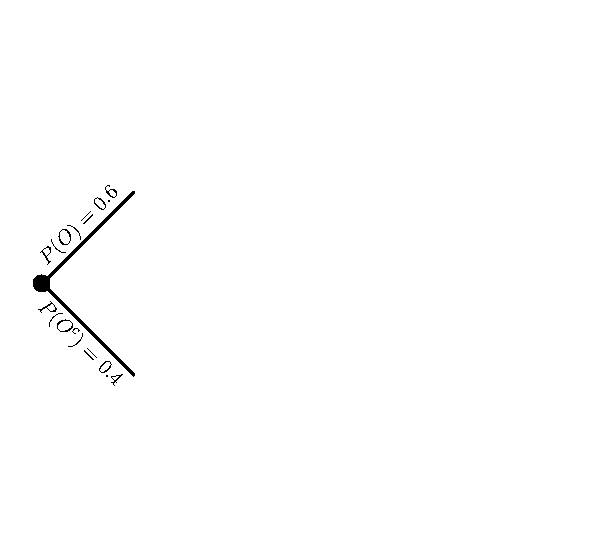
\includegraphics{chapters/chapter1/tree_diagram__branch1.pdf}}
    \caption{ }
\end{figure}

We pick the next event, say $D$, and create two branches from $O$ and two branches from $O^{c}$ for a total of four branches. 
Conditional on  $O$, two branches represent the occurrence of $D$ and occurrence of $D^{c}$.
Conditional on $O^{c}$, two branches represent the occurrence of $D$ and occurrence of $D^{c}$. 

\begin{figure}[ht!]
    \centering
    \fbox{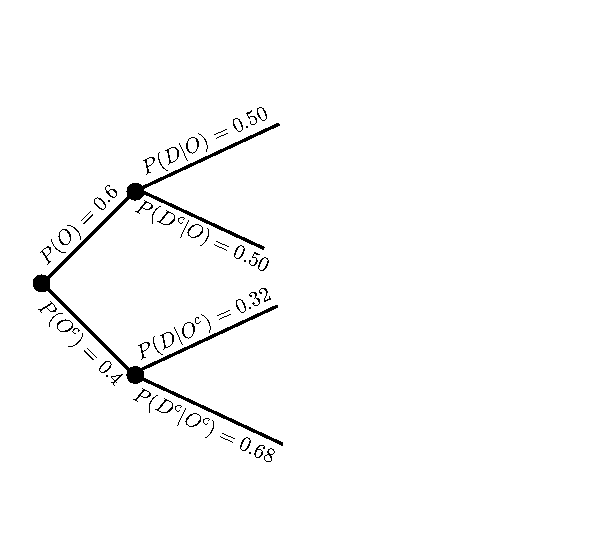
\includegraphics{chapters/chapter1/tree_diagram__branch2.pdf}}
    \caption{ }
\end{figure}

We can, in this example, do the same procedure for $S$ that we did for $D$, but this time we need to look at the occurrence of $S$ and $S^{c}$ for the four newest branches we created. 

\begin{figure}[ht!]
    \centering
    \fbox{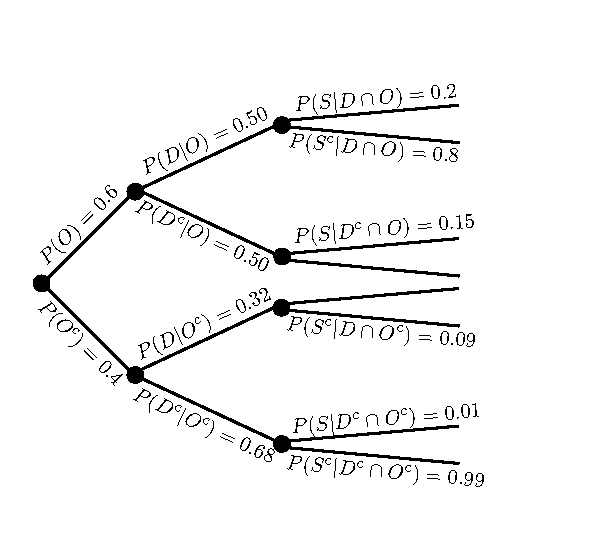
\includegraphics{chapters/chapter1/tree_diagram__branch3.pdf}}
    \caption{ }
\end{figure}


\clearpage
\subsubsection{Partitions and the law of total probability}

The multiplication rule is one way to use conditional probabilities to make computing probabilities of the intersection of many events more manageable.
We can also use conditional probabilities to simplify computing single events easier.

A \textbf{partition} of the event $A$ is a collection of sets $\mathcal{P} = \{B_{1}, B_{2}, \cdots, B_{n}\}$ such that $A = \left(A \cap B_{1}\right) \cup  \left(A \cap B_{2}\right)  \cup  \left(A \cap B_{3}\right) \cdots  \cup  \left(A \cap B_{n}\right)$ and for each $i,k$ pair of sets $B_{i} \cap B_{k} = \emptyset$.

\begin{figure}[ht!]
    \centering
    \fbox{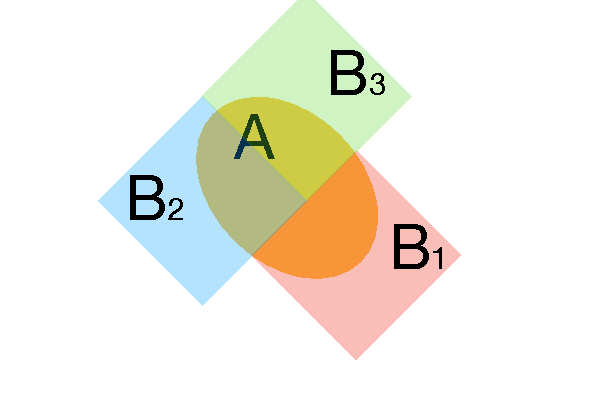
\includegraphics{chapters/chapter1/partition.pdf}}
    \caption{A partition $\mathcal{P} = \{B_{1},B_{2},B_{2}\}$ of the set $A$\label{fig.partition}}
\end{figure}


Because $B_{i}$ and $B_{k}$ are disjoint for any choice of $i$ and $k$, then $A \cap B_{i}$ and $A \cap B_{k}$ are also disjoint sets.
We can use the disjoint property of our partition to break down the probability of $A$ into the sum of probabilities of $A$ intersect $B_{k}$ for $k$ from $1$ to $n$.
\begin{align}
    P(A) &= P(\left(A \cap B_{1}\right) \cup  \left(A \cap B_{2}\right)  \cup  \left(A \cap B_{3}\right) \cdots  \cup  \left(A \cap B_{n}\right) \\
    &= P\left(A \cap B_{1}\right) +  P\left(A \cap B_{2}\right) +     + \cdots  +  P\left(A \cap B_{n}\right)  & \text{(Disjoint)}
\end{align}

We can further manipulate the above using the multiplication rule to find
\begin{align}
    P(A) &= P\left(A \cap B_{1}\right) +  P\left(A \cap B_{2}\right) +     + \cdots  +  P\left(A \cap B_{n}\right)  \\ 
         &= P(B_{1}) P(A|B_{1}) + P(B_{2}) P(A|B_{2}) + \cdots + P(B_{n}) P(A|B_{n}) 
\end{align}
This is called \textbf{the law of total probability}.
Intuitively the law of total probability says that the probability of an event $A$ can be computed by first considering the probabilities of a collection of related events, and then considering the probability that $A$ occurs given each related event. 

\ex Let $\mathcal{G} = \{(a,1), (a,2), (a,3), (b,4)\}$ and further suppose we assign the following probabilities to each outcome. 
\begin{table}[ht!]
    \centering
    \begin{tabular}{ll}
        Outcome & Probability \\
        \hline
        $(a,1)$ & 0.10\\
        $(a,2)$ & 0.25\\
        $(a,3)$ & 0.14\\
        $(b,4)$ & 0.51
    \end{tabular}
\end{table}

Define the events $A = \{ (a,1), (b,4), (a,2) \}$. The finest (as opposed to course) partition is a a collection of sets where each outcome in $A$ is in one, and only one, of the sets $B_{1},B_{2},...$. For example a partition of $A$ could be $\mathcal{P} = \{ B_{1}, B_{2}, B_{3} \}$ where $B_{1} = \{(a,1)\}$, $B_{2} = \{(b,4)\}$, and $B_{3} = \{(a,2)\}$. 
A courser partition is $\mathcal{P} = \{ B_{1}, B_{2} \}$ where $B_{1} = \{(a,1)\}$ and $B_{2} = \{(a,2),(b,4)\}$.



\subsubsection{Baye's Theorem}

We have investigated how the conditional probability is related to simultaneous events, gives us a natural definition of Independence, and can allow us to compute the probability of an event if we have a partition of that event. 

The final relationship we will explore is between two conditional probabilities. 

\textbf{Baye's Theorem} relates two conditional probabilities to one another 
\begin{align}
    P(A | B) =  \frac{P(B | A) P(A)}{P(B)}
\end{align}

We can show that Baye's theorem is true from the definition of conditional probability. 

\begin{align}
    &P(A | B) = \frac{P(A \cap B)}{P(B)}  & \text{definition} \\ 
    &P(A | B) = \frac{P(B |A) P(A)}{P(B)} & \text{multiplication rule} 
\end{align}



\subsubsection{Repeated experiments}
Many natural experiments involve repeated observations. 
It may be of interest to observe the whether and assign a probability to "sunny" or "cloudy" weather conditions. 
However, many vacationers, who plan to spend 2, 3, or more days at a remote destination may want to know the probability that the next $X$ days are sunny. 

The Cartesian product gives us a natural way to express repeated experiments.
If we chose to repeat an experiment $N$ times where each experiment produced an outcome in $\mathcal{G}$, we could imagine the set of outcomes as tuples of length $N$ where each entry in the tuple is from our sample space.
In other words, a single outcome in this repeated experiment would be $(o_{1},o_{2},o_{3},\cdots,o_{N})$ and this outcome is a member of the set $\mathcal{G} \times \mathcal{G} \times \mathcal{G} \times \cdots \times \mathcal{G}$.

Back to our vacation example. 
If a vacationer wanted to understand the chances they had of enjoying $5$ sunny days in a row, then we know that we could defined a sample space $\mathcal{G} = \{\text{"sunny"},\text{"not sunny"}\}$ and we also know that the vacationer is interested in outcomes in the sample space 
\begin{equation}
    (d_{1},d_{2},d_{3},d_{4},d_{5}) \in \mathcal{G} \times \mathcal{G}\times \mathcal{G}\times \mathcal{G}\times \mathcal{G} 
\end{equation}
where $d_{i}$ is the outcome on day $i$.
We can frame the problem, and clearly layout the potential outcomes, for example on outcome is ("sunny", "sunny", "not sunny", "sunny", "not sunny").

\subsection{The datapoint, dataset, and dataframe}

The sample space, event, and outcome are all potential results from an experiment. 
When we conduct an experiment we will generate an outcome from our sample space and call this realized outcome a \textbf{data point}. 

\ex Consider the experiment of flipping a coin and recording whether the coin lands heads or tails side up.
We can define a sample space $\samplespace = \{H,T\}$ where $H$ is an outcome that represents the coin landing heads up and $T$ represents tails up. Up until this point we have structured our experiment, but we have generated no data. We flip the coin and the coin lands tails side up. Now we have performed an experiment and generated the data point $T$.

Now suppose that we conduct an experiment with the same sample space~$(\samplespace)$ a number $N$ times and with each experiment we record a data point. A tuple of data points~$d$ is called a \textbf{data set}~$\mathcal{D} = (d_{1}, d_{2}, d_{3}, \cdots, d_{N})$ where $d_{i}$ is the data point generated from the $i^\text{th}$ experiment.
We say that we have \underline{drawn} or that we have \underline{sampled} a data set $\mathcal{D}$. Further, data points~$(d)$ are often called \underline{realized} outcomes because they are no longer in a set of potential possibilities but are now determined items. 

A data set~$\mathcal{D}$ can be unwieldy depending on the number of data points, the complexity of the sample space, or both.
A \textbf{data frame} is one way to organize a data set.
A data frame~$\mathcal{F}$ is a table where each data point~$d$ in a dataset~$\mathcal{D}$ is represented as a row in the table and if the data point is a tuple then a separate column is created for each position in the tuple.

\ex Suppose we design an experiment to collect from humans predictions, two weeks ahead from the time of our experiment, of the number of incident cases and incident deaths at the US national level of COVID-19~(\url{https://www.ncbi.nlm.nih.gov/pmc/articles/PMC7523166/}). We decide to collect from each human whether they are an expert in the modeling of infectious disease,  a prediction of incident cases, and a prediction of incident deaths. We draw a data set $\mathcal{D}$ of 50 human judgement predictions. We can organize this data set into a data frame 
\begin{table}[ht!]
    \centering
    \begin{tabular}{c|c|c}
    Expert & Prediction of cases & Prediction of deaths\\
    \hline
    Yes     & 145    & 52 \\ 
    No      & 215    & 34 \\
    Yes     & 524    & 48 \\
    Yes     & 265    & 95 \\
    No      & 354    & 35 \\
    \end{tabular}
    \caption{Example data frame $\mathcal{F}$ built from a data set~$\mathcal{D}$ that contains 5 data points where each data point is a tuple of length three.}
\end{table}

Above, the first data point is $(Yes,145,52)$, the second data point is $(No, 215, 34)$, and so on until the last data point $(No, 354, 35)$. A data frame can also include informative information for others such as labels for each column.


\section{Exercises}

\begin{enumerate}
    \item \begin{align*}
              A &= \{1,2,3,4,5,6\};
              \;\;B = \{1,3,6\} \\
              C &= \{7\}  
              \;\;D = \emptyset
           \end{align*}
    \begin{enumerate}
        \item Please compute $A \cap B$
        \item Please compute $A \cup C$
        \item Please compute $A \cup D$
        \item Please compute $A \cap D$
        \item Please compute $(A \cap B) \cup (C \cup D)$
    \end{enumerate}
    \item Let the sample space $\mathcal{G} = \{ 1,2,3,4,5,6,7 \}$
    \begin{enumerate}
       \item Please compute $A^{c}$
       \item Please compute $B^{c}$
       \item Please compute $D^{c}$
       \item Please compute $\mathcal{G} \cap A$
       \item Is $A \subset \mathcal{G}$?
       \item Is $\emptyset \subset \mathcal{G}$?
    \end{enumerate}
    
    \item Let the sample space $\samplespace = \{0,1,2,a,b,c\}$ and let $A=\{0,1\}$, $B=\{x | x\text{ is a letter of the English alphabet}\}$
    \begin{enumerate}
        \item Please compute $A \cap B$
        \item Please compute $A \cup B$
        \item Please compute $A^{c}$
        \item Is $A \cup B = \samplespace$?
        \item If we assigned probabilities to all outcomes, could $P(A \cup B) = 1$? why or why not?
    \end{enumerate}
    
    \item Let $A = {0,1,2}$ for some sample space $\mathcal{G} = \{0,1,2,3,4,5,6\}$. Further assume $P(A) = 0.2$. 
    \begin{enumerate}
        \item Are the sets $A$ and $A^{c}$ disjoint? Why or why not.
        \item Simplify $P(A \cup A^{c})$ into an expression that involves $P(A)$ and $P(A^{c})$.
        \item Use Kolmogorov's axioms to show that $P(A) = 1 - P(A^{c})$ 
    \end{enumerate}
    
    \item Let $\samplespace = \{x | x\text{ is a positive integer}\}$
    \begin{enumerate}
        \item Are the sets $\emptyset$ and $\samplespace$ disjoint?
        \item Simplify $P(\samplespace \cup \emptyset)$ into an expression that involves $P(\samplespace)$ and $P(\emptyset)$
        \item Use Kolmogorov's axioms to show that $P(\emptyset) = 0$
    \end{enumerate}
    
    \item If $A=\{1,2,3\}$ and $B = \{2,3,4\}$ and $C = \{1,3\}$
    \begin{enumerate}
        \item Can $P(A) < P(B)$? Why or why not
        \item Can $P(A) < P(C)$? Why or why not
    \end{enumerate}
    \item Use what you know about the intersection, about subsets, and about probability to show that $P(A \cap B) \leq P(A)$. Hint: How are $A \cap B$ and $A$ related?
    \item Suppose we wish to study the reemergence of cancer among patients in remition. We collect data on 1,000 patients who are in cancer remition and follow them for 5 years. At five years we are interested in the probability of a second cancer. 
    \begin{enumerate}
        \item Define a sample space $\mathcal{G}$ we can use to assign probabilities to a second cancer and no second cancer. 
        \item After five years of followup we find that 238 patients experienced a second cancer. Use the frequentist approach to assign probabilities to a second cancer \underline{and} no second cancer.
        \item If you collected data on 2,000 patients do you expect the probability of a second cancer to change? How do you expect the probability to be different for 2,000 patients than with 1,000 patients? 
    \end{enumerate}
    
   \item A study (link = \href{here}{https://www.science.org/doi/10.1126/science.abj8222} found that young adults were 32 times more at risk to develop multiple sclerosis (MS) after infection with the Epstein-Barr virus compared to young adults who were not infected by the virus. The experiment enrolled 10 million young adults and observed them for a period of 20 years.
   \begin{enumerate}
       \item Design a sample space if we wish to study outcomes that describe the number of young adults who develop MS. 
       \item Build the event $(E_{1})$ "less than 10\% of young adults develop MS" using set notation.
       \item Build the event $(E_{2})$ "less than 5\% of young adults develop MS" using set notation.
       \item Are $E_{1}$ and $E_{2}$ disjoint? Why or why not?
       \item Can $P(E_{1}) < P(E_{2})$?
   \end{enumerate}
   
   \item Please compute the following
   \begin{enumerate}
       \item $A = \{1,2,3\}$ and $B = \{4,5,6\}$. Please compute $A \times B$ (Answer should be a set of tuples)
       \item $A = \{1,2,3\}$. Please compute $A \times A$ (Answer should be a set of tuples)
       \item How many elements are in $A \times A$ (looking for a number)
       \item How many elements are in  $A \times A \times A$? (looking for a number)
       \item How many elements are in  $A \times A \times A \times \cdots \times A$ where we take the Cartesian product $N$ times? (looking for a number)
   \end{enumerate}
   \item Define a sample space $\samplespace = \{ a,b,c,d,1,2,3,4,5 \}$ and let $E_{1} = \{1,3,5\}$, $E_{2} = \{a,b,c\}$, $E_{3} = \{ a,d,5 \}$. We further assign the following probabilities 
   \begin{table}[ht!]
       \centering
       \begin{tabular}{ c c}
       Outcome &  $P(\{\text{Outcome}\})$\\
       \hline
            a & 0.10  \\
            b & 0.05 \\
            c & 0.15 \\
            d & 0.02 \\
            1 & 0.14 \\
            2 & 0.25 \\
            3 & 0.08 \\
            4 & 0.04 \\
            5 & 0.17
       \end{tabular}
   \end{table}
   \begin{enumerate}
       \item Compute $P(E_{1})$ (looking for a number)
       \item Compute $P(E_{2})$ (looking for a number)
       \item Compute $P(E_{3})$ (looking for a number)
       \item Compute $P(E_{1} \cap E_{2})$ (looking for a number)
       \item Compute $P(E_{1} \cap E_{3})$ (looking for a number)
       \item Compute $P(E_{2} \cap E_{3})$ (looking for a number)
       \item Compute $P(E_{1} | E_{2})$ (looking for a number)
       \item Compute $P(E_{1} | E_{3})$ (looking for a number)
       \item Compute $P(E_{2} | E_{3})$ (looking for a number)
       \item Compute $P(E_{3} | E_{2})$ (looking for a number)
   \end{enumerate}
   \item Define a sample space $\samplespace = \{ (a,1),(b,1),(c,1),(a,2),(b,2),(c,2) \}$ and let $E_{1} = \{(a,1),(a,2),(c,2)\}$, $E_{2} = \{(c,2),(a,1) \}$, $E_{3} = \{(b,2) \}$. We further assign the following probabilities 
   \begin{table}[ht!]
       \centering
       \begin{tabular}{ c c}
       Outcome &  $P(\{\text{Outcome}\})$\\
       \hline
            (a,1) & 0.05  \\
            (b,1) & 0.22 \\
            (c,1) & 0.15 \\
            (a,2) & 0.02 \\
            (b,2) & 0.13 \\
            (c,2) & 0.43 \\
       \end{tabular}
   \end{table}
   \begin{enumerate}
       \item Compute $P(E_{1})$ (looking for a number)
       \item Compute $P(E_{2})$ (looking for a number)
       \item Compute $P(E_{3})$ (looking for a number)
       \item Compute $P(E_{1} \cap E_{2})$ (looking for a number)
       \item Compute $P(E_{1} \cap E_{3})$ (looking for a number)
       \item Compute $P(E_{2} \cap E_{3})$ (looking for a number)
       \item Compute $P(E_{1} | E_{2})$ (looking for a number)
       \item Compute $P(E_{1} | E_{3})$ (looking for a number)
       \item Compute $P(E_{2} | E_{3})$ (looking for a number)
       \item Compute $P(E_{3} | E_{2})$ (looking for a number)
   \end{enumerate}
   
   \item Given two events $A$ and $B$, show that $P(A|B) \geq P(A \cap B)$ (looking for a short explanation and mathematical argument)
   
   \item Suppose we wish to study adverse outcomes among patients who have unprotected left main disease~(\url{https://www.nejm.org/doi/full/10.1056/nejmoa1909406}). In this experiment~(called a clinical trial) we randomize patients to receive percutaneous intervention~(PCI) or a coronary artery bypass graft~(CABG). We wish to study the number of patients who received a PCI \underline{and} experienced a myocardial infarction~(MI) between the time they had their procedure and 5 years, however we only know three pieces of information: (i) the probability a patient was randomized to PCI was 0.5, (ii) the probability a patient was randomized to CABG was 0.5, and (iii) we know that the probability of a MI was 0.2 among patients who received a PCI.
   \begin{enumerate}
       \item Define a sample space that will allow us to compute the probability a patient was randomized to PCI and experienced an MI (looking for a description of the sample space and a set)
       \item Please compute the probability a patient experiences an MI and was randomized to PCI. (looking for a number)
       \item Please compute the probability a patient does not experience an MI and was randomized to PCI. (looking for a number)
   \end{enumerate}
   
   \item If two events $A$ and $B$ are disjoint, are they also independent? (looking for a description and mathematical argument to backup your description.)
   
   \item Researchers studied epidemiological characteristics of a variant of SARS-CoV-2 called B.1.526~(\url{https://www.science.org/doi/10.1126/sciadv.abm0300}). Suppose we too wanted to study the impact of B.1.526 on a population of patients who have been admitted to the hospital for COVID-19 by collecting each patient's age, whether they have were vaccinated against COVID-19, and whether their infection was due to the B.1.526 variant.
   
   \begin{enumerate}
       \item If we define our experiment as generating the above three pieces of information from a single patient, define a sample space~($\samplespace$) for these potential outcomes. (looking for a short description and the sample space)
       \item Define a sample space if we repeated our above experiment 2 times. In other words, what would be our sample space if we collected information from 2 patients? 
   \end{enumerate}
    
   \item Can a data set ever have more elements than a sample space? Explain. (looking for a paragraph with some examples)
   
   \item Suppose we collect the following data about the co-occurence of patients admitted to the hospital for influenza-like illness~(ILI) and whether the patient does or does not work in a clinical setting. 
   After data collection we estimate the following probabilities: The probability that a patient works in a clinical setting is 0.12. The probability that a patient who works in a clinical setting is admitted to the hospital for ILI is 0.2, and the probability a patient who does not work in a clinical setting was admitted to the hospital for ILI is 0.3. 
   \begin{enumerate}
       \item Define a sample space to study outcomes related to the co-occurance of ILI/No ILI and patients who do/do not work in a clinical setting. (Looking for a set and a very brief description of an outcome or two.) 
       \item Compute the probability a patient is admitted to the hospitals for ILI and they work in a clinical setting. (Looking for an equation and number)
       \item Compute the probability a patient is not admitted to the hospital for ILI and they work in a clinical setting. (Looking for an equation and number)
       \item Compute the probability a patient is admitted to the hospital for ILI and they do not work in a clinical setting. (Looking for an equation and number)
       \item Compute the probability a patient is not admitted to the hospital for ILI and they do not work in a clinical setting. (Looking for an equation and number)
   \end{enumerate}
   
   \item Show that for two events $A$ and $B$ the $P(A|B)P(B)  \leq P(B)$. Why is this the case intuitively? (Looking for two brief descriptions)
   \clearpage
   \item \begin{figure}[ht!]
       \centering
       \fbox{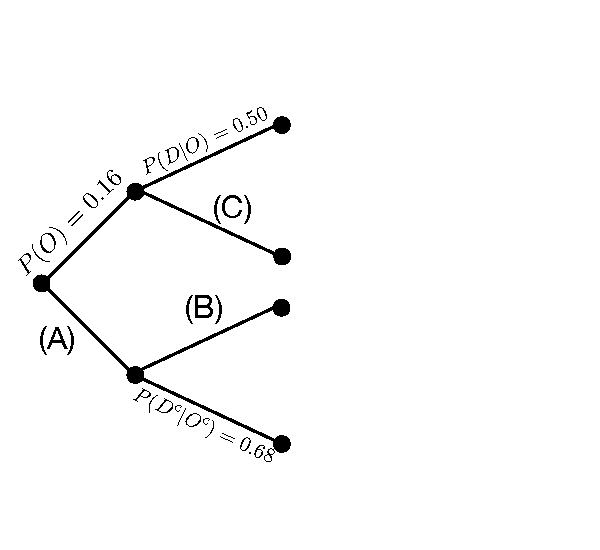
\includegraphics{chapters/chapter1/tree_diagram__HW.pdf}}
   \end{figure} Please use the above tree diagram to answer the following questions. 
   \begin{enumerate}
       \item Fill in the $P(O^{c})$ which corresponds to (A) in the figure
       \item Fill in the $P(D | O^{c})$ which corresponds to (B) in the figure
       \item Fill in the $P(D^{c} | O)$ which corresponds to (C) in the figure
       \item Please compute $P(D)$
       \item Please compute $P(D^{c})$
   \end{enumerate}
   
   \item Influenza is a contagious virus that enters the respiratory system from a human's nose, throat, or lungs. Common symptoms are cough, chills, and a fever.
   Suppose we collect data from a local hospital about those who were infected and not infected by the influenza virus and the above three symptoms. Let $\samplespace = \{ (x,y)  | x \text{ is } \text{"Flu"} \text{ or } \text{"not Flu"} \text{ and } y \in \{ \text{cough },\text{chills },\text{ fever} \}   \}$. 
   Suppose further that we define events $F$ = \{ (x,y)  | x \text{ is } \text{"Flu"} \}, $C$ = \{ (x,y)  | y \text{ is } \text{"Cough"} \}, $H$ = \{ (x,y)  | y \text{ is } \text{"Chills"} \} , $E$ = \{ (x,y)  | y \text{ is } \text{"Fever"} \}, and that $P( C|F ) = 0.5$ and $P( C|F^{c} ) = 0.15$, $P( H|F ) = 0.25$ and $P( H|F^{c} ) = 0.01$, $P( E|F ) = 0.98$ and $P( E|F^{c} ) = 0.35$, $P(F) = 0.02$  
    \begin{enumerate}
       \item A patient presents with the chills. What is the probability they have influenza? 
       \item What symptom from the above, if present, would indicate with a high probability a patient has influenza?
    \end{enumerate}
    
\end{enumerate}

\section{Student contributions}


\textit{Jessica Berman - Class of 2025-Advice:} When I see a problem pertaining to conditional probability it helps me to talk the question out and actually say to myself “what is the probability of A given B has already occured” because P(A|B) is not clear to me without saying it aloud.

\textit{Jessica Berman - Class of 2025-Example:} A fun fact about conditional probability is that it is used in politics. For example, if there are 4 candidates running in a presidential election, the chances of winning for each of them is 25%. However, given that one candidate drops out of the race two weeks later, the candidates' probability of winning changes to 33.33% each (P(Win | One candidate drops out)).


\textit{Monelli Esfandiary---Class of 2025---Insight:}
PELO assumes you assign the same probability to every outcome in your sample space.
The frequentist approach assigns a probability to each outcome that is proportional to the number of times we observe that outcome in a dataset.
Though the PELO and Frequentist approach appear different, we can show that the PELO is a special case of the Frequentist approach. 
Suppose we create a sample space $\mathcal{G} = \{H,T\}$.
PELO would assign P(\{$H$\}) = $C$ and P(\{$T$\}) = $C$, and so (1 = $2C$) = (0.5 = $C$). 
But we could arrive at the same result using the Frequentist approach if we sampled every outcome from $\mathcal{G}$ once. 


\textit{Anyah Kumar---Class of 2025---Statistical Independence:} The topic from chapter one that I liked the most was statistical independence.
Two events, $A$ and $B$, are statistically independent when one probability does not affect the probability of the other.
This may remind you of mutually exclusive events. However, mutually exclusive events cannot be statically independent because when one event occurs the other event \textbf{CANNOT} occur. 
That's why I like statistical independence, because the probability of one event doesn't change the probability of another event which makes computing the probability of the two events simpler.


\section{Glossary}
\begin{Glossary}
\item[Set]
\item[Subset]
\item[Set equality]
\item[Set intersection]
\item[Set union]
\item[Universal set]
\item[Empty set]
\item[Sample space]
\item[Experiment]
\item[Outcome]
\item[Event]
\item[Probability]
\item[Kolmorogov's Axioms]
\item[Principle of Equally Likely Outcomes]
\item[Product Set]
\item[Compound event]
\item[Conditional probability]
\item[Multiplication Rule]
\item[Independence]
\end{Glossary}






